\begin{frame}
  \frametitle{Porting the Linux kernel}
  \begin{itemize}
  \item The Linux kernel supports a lot of different CPU architectures
  \item Each of them is maintained by a different group of
    contributors
    \begin{itemize}
    \item See the \kpath{MAINTAINERS} file for details
    \end{itemize}
  \item The organization of the source code and the methods to port
    the Linux kernel to a new board are therefore very
    architecture-dependent
    \begin{itemize}
    \item For example, some architectures use the Device Tree, some do
      not.
    \end{itemize}
  \item This presentation is focused on the ARM architecture only
  \end{itemize}
\end{frame}

\begin{frame}
  \frametitle{Architecture, CPU and Machine}
  \begin{itemize}
  \item In the source tree, each architecture has its own directory
    \begin{itemize}
    \item \kpath{arch/arm} for the ARM architecture
    \end{itemize}
  \item This directory contains generic ARM code
    \begin{itemize}
    \item \code{boot}, \code{common}, \code{configs}, \code{kernel},
      \code{lib}, \code{mm}, \code{nwfpe}, \code{vfp},
      \code{oprofile}, \code{tools}
    \end{itemize}
  \item And many directories for different SoC families
    \begin{itemize}
    \item \code{mach-*} directories: \code{mach-pxa} for PXA CPUs,
      \code{mach-imx} for Freescale iMX CPUs, etc.
      \begin{itemize}
      \item Before the ARM cleanup, those directories contained
        support for the SoC family (GPIO, clocks, pinmux, power
        management, interrupt controller, etc.) and for the various
        boards.
      \item Nowadays, they contain a lot less code, essentially a
        small SoC description file, power management and SMP code.
      \end{itemize}
    \end{itemize}
  \item Some CPU types share some code, in directories named
    \code{plat-*}
  \item Device Tree files in \kpath{arch/arm/boot/dts}.
  \end{itemize}
\end{frame}

\begin{frame}
  \frametitle{Before the Device Tree and ARM cleanup}
  \begin{itemize}
  \item Until 2011, the ARM architecture wasn't using the Device Tree,
    and a large portion of the SoC support was located in
    \code{arch/arm/mach-<foo>}.
  \item Each board supported by the kernel was associated to an unique
    {\em machine ID}.
  \item The entire list of {\em machine ID} can be downloaded at
    \url{http://www.arm.linux.org.uk/developer/machines/download.php}
    and one could freely register an additional one.
  \item The Linux kernel was defining a {\em machine structure} for
    each board, which associates the {\em machine ID} with a set of
    information and callbacks.
  \item The bootloader had to pass the {\em machine ID} to the kernel
    in a specific ARM register.
  \end{itemize}
\end{frame}

\begin{frame}
  \frametitle{The Device Tree and the ARM cleanup}
  \begin{itemize}
  \item As the ARM architecture gained significantly in popularity,
    some major refactoring was needed.
  \item First, the Device Tree was introduced on ARM: instead of using
    C code to describe SoCs and boards, a specialized language is
    used.
  \item Second, many driver infrastructures were created to replace
    custom code in \code{arch/arm/mach-<foo>}:
    \begin{itemize}
    \item The common clock framework in \kpath{drivers/clk}
    \item The pinctrl subsystem in \kpath{drivers/pinctrl}
    \item The irqchip subsystem in \kpath{drivers/irqchip}
    \item The clocksource subsystem in \kpath{drivers/clocksource}
    \end{itemize}
  \item The amount of code in \code{mach-<foo>} has now significantly
    reduced.
  \end{itemize}
\end{frame}

\begin{frame}
  \frametitle{Adding the support for a new ARM board}
  Provided the SoC used on your board is supported by the Linux kernel:
  \begin{enumerate}
  \item Create a {\em Device Tree} file in \kpath{arch/arm/boot/dts},
    generally named \code{<soc-name>-<board-name>.dts}, and make it
    include the relevant SoC \code{.dtsi} file.
    \begin{itemize}
    \item Your Device Tree will describe all the SoC peripherals that
      are enabled, the pin muxing, as well as all the devices on the
      board.
    \end{itemize}
  \item Modify \kpath{arch/arm/boot/dts/Makefile} to make sure your
    Device Tree gets built as a {\em DTB} during the kernel build.
  \item If needed, develop the missing device drivers for the devices
    that are on your board outside the SoC.
  \end{enumerate}
\end{frame}

\begin{frame}
  \frametitle{Example of the Freescale iMX28 SoCs}
  \begin{itemize}
  \item The hardware platform used in this training is based on the
    AM335x processor from Texas Instruments.
  \item This platform inherits from the OMAP family of TI, for which
    kernel support has been around for a long time.
  \item Due to this, and the complexity of the platform, the AM335x
    and OMAP support in the kernel hasn't fully migrated yet to all
    the infrastructures created during the {\em ARM cleanup}.
  \item Therefore, to illustrate this section, we will take the
    example of the Freescale iMX28 platform, on which Free Electrons
    has worked specifically.
  \end{itemize}
\end{frame}

\begin{frame}
  \frametitle{Studying the Crystalfontz CFA-10036 platform}
  \begin{columns}
    \column{0.7\textwidth}
    \begin{itemize}
    \item Crystalfontz CFA-10036
    \item Uses the Freescale iMX28 SoC, from the MXS family.
    \item 128MB of RAM
    \item 1 serial port, 1 LED
    \item 1 I2C bus, equipped with an OLED display
    \item 1 SD-Card slot
    \end{itemize}
    \column{0.3\textwidth}
    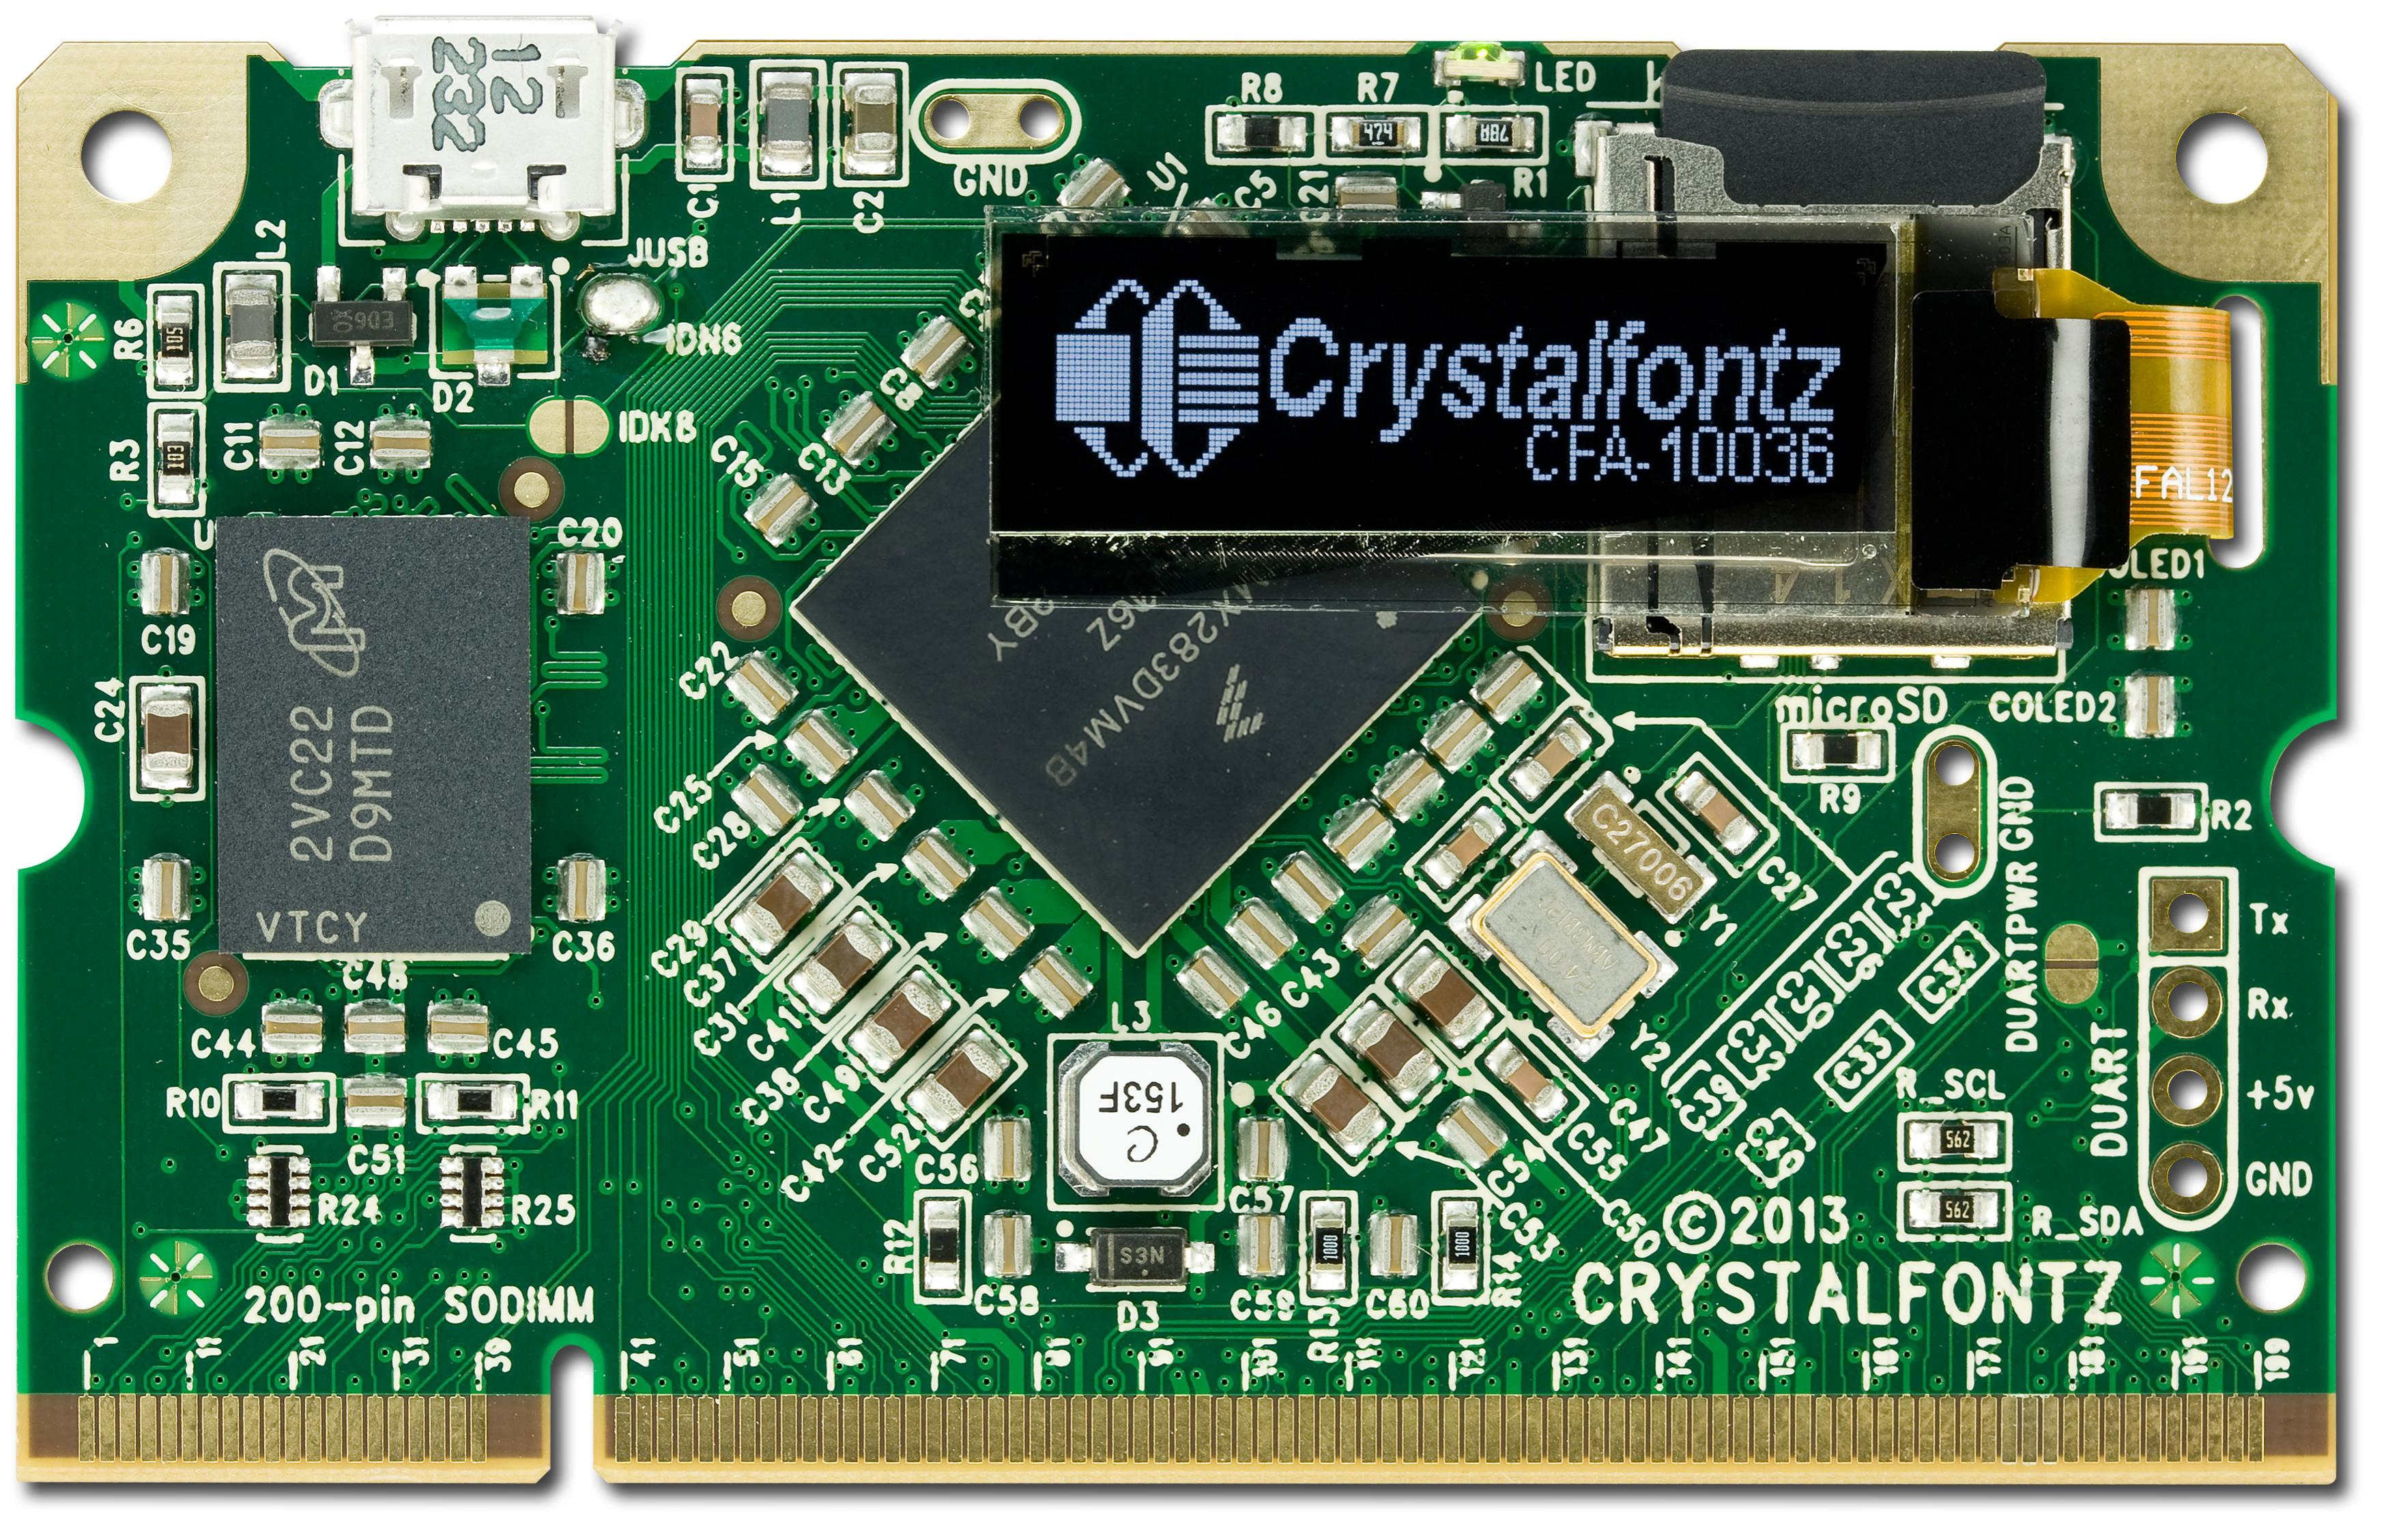
\includegraphics[width=\textwidth]{slides/kernel-porting-content/crystalfontz.jpg}
  \end{columns}
\end{frame}

\begin{frame}[fragile]
  \frametitle{Crystalfontz CFA-10036 Device Tree, header}
  \begin{itemize}
  \item Mandatory Device Tree language definition\\
    \begin{block}{} \mint[fontsize=\tiny]{perl}+/dts-v1/+ \end{block}
  \item Include the \code{.dtsi} file describing the SoC\\
    \begin{block}{}
      \mint[fontsize=\tiny]{perl}+#include "im28.dtsi"+
    \end{block}
  \item Start the root of the tree\\
    \begin{block}{} \mint[fontsize=\tiny]{perl}+/ {+ \end{block}
  \item A human-readable string to describe the machine\\
    \begin{block}{}
      \mint[fontsize=\tiny]{perl}+model = "Crystalfontz CFA-10036 Board";+
    \end{block}
  \item A list of {\em compatible} strings, from the most specific one
    to the most general one. Can be used by kernel code to do a SoC or
    board-specific check.\\
    \begin{block}{}
      \mint[fontsize=\tiny]{perl}+compatible = "crystalfontz,cfa10036", "fsl,imx28";+
    \end{block}
  \end{itemize}
\end{frame}

\begin{frame}[fragile]
  \frametitle{Crystalfontz CFA-10036 Device Tree, chosen/memory}
  \begin{itemize}
  \item Definition of the default {\em kernel command line}. Some
    additional operating-system specific entries can be added in
    \code{chosen}:
    \begin{block}{}
    \begin{minted}[fontsize=\footnotesize]{perl}
chosen {
        bootargs = "console=ttyS0,115200 earlyprintk";
};
\end{minted}
\end{block}
\item Definition of the size and location of the RAM:
  \begin{block}{}
    \begin{minted}[fontsize=\footnotesize]{perl}
memory {
        device_type = "memory";
        reg = <0x40000000 0x8000000>; /* 128 MB */
};
      \end{minted}
    \end{block}
  \end{itemize}
\end{frame}

\begin{frame}[fragile]
  \frametitle{Crystalfontz CFA-10036, bus/UART}
  \begin{itemize}
  \item Start of the internal SoC peripherals.
    \begin{block}{}
    \begin{minted}[fontsize=\tiny]{perl}
apb@80000000 {
    apbh@80000000 {
        apbx@80040000 {
\end{minted}
\end{block}
\item The CFA-10036 has one debug UART, so the corresponding
  controller is enabled:
  \begin{block}{}
    \begin{minted}[fontsize=\tiny]{perl}
duart: serial@80074000 {
    pinctrl-names = "default";
    pinctrl-0 = <&duart_pins_b>;
    status = "okay";
};
    \end{minted}
  \end{block}
\end{itemize}
\end{frame}

\begin{frame}[fragile]
  \frametitle{Crystalfontz CFA-10036 Device Tree, Muxing}
\begin{itemize}
  \item Definition of a few pins that will be muxed as GPIO, for LEDs and reset.
  \begin{block}{}
    \begin{minted}[fontsize=\tiny]{perl}
pinctrl@80018000 {
    ssd1306_cfa10036: ssd1306-10036@0 {
        reg = <0>;
        fsl,pinmux-ids = <
            0x2073 /* MX28_PAD_SSP0_D7__GPIO_2_7 */
        >;
        fsl,drive-strength = <0>;
        fsl,voltage = <1>;
        fsl,pull-up = <0>;
    };

    led_pins_cfa10036: leds-10036@0 {
        reg = <0>;
        fsl,pinmux-ids = <
            0x3043 /* MX28_PAD_AUART1_RX__GPIO_3_4 */
        >;
        fsl,drive-strength = <0>;
        fsl,voltage = <1>;
        fsl,pull-up = <0>;
    };
};
    \end{minted}
  \end{block}
  \end{itemize}
\end{frame}

\begin{frame}[fragile]
  \frametitle{Crystalfontz CFA-10036 Device Tree, LED}
\begin{itemize}
\item One LED is connected to this platform. Note the reference to the
  \code{led_pins_cfa10036} muxing configuration.
  \begin{block}{}
    \begin{minted}[fontsize=\tiny]{perl}
leds {
    compatible = "gpio-leds";
    pinctrl-names = "default";
    pinctrl-0 = <&led_pins_cfa10036>;

    power {
        gpios = <&gpio3 4 1>;
        default-state = "on";
    };
};
    \end{minted}
    \end{block}
  \end{itemize}
\end{frame}

\begin{frame}[fragile]
  \frametitle{Crystalfontz CFA-10036 Device Tree, SD Card/USB}
  \begin{itemize}
  \item The platform also has a USB port
    \begin{block}{}
      \begin{minted}[fontsize=\tiny]{perl}
usb0: usb@80080000 {
    pinctrl-names = "default";
    pinctrl-0 = <&usb0_otg_cfa10036>;
    status = "okay";
};
      \end{minted}
    \end{block}
  \item and an SD Card slot:
    \begin{block}{}
      \begin{minted}[fontsize=\tiny]{perl}
ssp0: ssp@80010000 {
    compatible = "fsl,imx28-mmc";
    pinctrl-names = "default";
    pinctrl-0 = <&mmc0_4bit_pins_a
                 &mmc0_cd_cfg &mmc0_sck_cfg>;
    bus-width = <4>;
    status = "okay";
};
    \end{minted}
    \end{block}
  \end{itemize}
\end{frame}

\begin{frame}[fragile]
  \frametitle{Crystalfontz CFA-10036 Device Tree, I2C bus}
  \begin{itemize}
  \item An I2C bus, with a Solomon SSD1306 OLED display connected on
    it:
    \begin{block}{}
      \begin{minted}[fontsize=\tiny]{perl}
i2c0: i2c@80058000 {
    pinctrl-names = "default";
    pinctrl-0 = <&i2c0_pins_b>;
    clock-frequency = <400000>;
    status = "okay";

    ssd1306: oled@3c {
        compatible = "solomon,ssd1306fb-i2c";
        pinctrl-names = "default";
        pinctrl-0 = <&ssd1306_cfa10036>;
        reg = <0x3c>;
        reset-gpios = <&gpio2 7 0>;
        solomon,height = <32>;
        solomon,width = <128>;
        solomon,page-offset = <0>;
    };
};
      \end{minted}
    \end{block}
  \end{itemize}
\end{frame}

\begin{frame}[fragile]
  \frametitle{Crystalfontz CFA-10036 Device Tree, Breakout Boards}
  \begin{itemize}
  \item The CFA-10036 can be plugged in other breakout boards, and the
    device tree also allows us to describe this, using includes. For
    example, the CFA-10057:
    \begin{block}{}
      \mint[fontsize=\tiny]{perl}+#include "imx28-cfa10036.dts"+
    \end{block}
  \item This allows to have a layered description. This can also be
    done for boards that have a lot in common, like the BeagleBone and
    the BeagleBone Black, or the AT91 SAMA5D3-based boards.
  \end{itemize}
\end{frame}

\begin{frame}[fragile]
  \frametitle{Crystalfontz CFA-10036: build the DTB}
  \begin{itemize}
  \item To ensure that the Device Tree Blob gets built for this board
    Device Tree Source, one need to ensure it is listed in
    \kpath{arch/arm/boot/dts/Makefile}:
    \begin{block}{}
      \begin{minted}{make}
dtb-$(CONFIG_ARCH_MXS) += imx28-cfa10036.dtb \
        imx28-cfa10037.dtb \
        imx28-cfa10049.dtb \
        imx28-cfa10055.dtb \
        imx28-cfa10056.dtb \
        imx28-cfa10057.dtb \
        imx28-cfa10058.dtb \
        imx28-evk.dtb
      \end{minted}
    \end{block}
  \end{itemize}
\end{frame}

\begin{frame}
  \frametitle{Understanding the SoC support}
  \begin{itemize}
  \item Let's consider another ARM platform here, the Marvell Armada
    370/XP.
  \item For this platform, the core of the SoC support is located in
    \kpath{arch/arm/mach-mvebu}
  \item The \code{armada-370-xp.c} (see code on the next slide)
    contains the "{\em entry point}" of the SoC definition, the
    \code{DT_MACHINE_START} .. \code{MACHINE_END} definition:
    \begin{itemize}
    \item Defines the list of platform compatible strings that will
      match this platform, in this case
      \code{marvell,armada-370-xp}. This allows the kernel to know
      which \code{DT_MACHINE} structure to use depending on the DTB
      that is passed at boot time.
    \item Defines various callbacks for the platform initialization,
      the most important one being the \code{.init_machine} callback,
      which calls \kfunc{of_platform_populate}. This function travels
      through the Device Tree and instantiates all the devices.
    \end{itemize}
  \end{itemize}
\end{frame}

\begin{frame}[fragile]
  \frametitle{{\tt arch/arm/mach-mvebu/armada-370-xp.c}}
  \begin{block}{}
    \begin{minted}[fontsize=\tiny]{c}
static void __init armada_370_xp_dt_init(void)
{
        of_platform_populate(NULL, of_default_bus_match_table, NULL, NULL);
}

static const char * const armada_370_xp_dt_compat[] = {
        "marvell,armada-370-xp",
        NULL,
};

DT_MACHINE_START(ARMADA_XP_DT, "Marvell Armada 370/XP (Device Tree)")
        .smp            = smp_ops(armada_xp_smp_ops),
        .init_machine   = armada_370_xp_dt_init,
        .map_io         = armada_370_xp_map_io,
        .init_time      = armada_370_xp_timer_and_clk_init,
        .restart        = mvebu_restart,
        .dt_compat      = armada_370_xp_dt_compat,
MACHINE_END
  \end{minted}
 \end{block}
\end{frame}

\begin{frame}
  \frametitle{Components of the minimal SoC support}
  The minimal SoC support consists in
  \footnotesize
  \begin{itemize}
  \item An SoC {\em entry point} file,
    \kpath{arch/arm/mach-mvebu/armada-370-xp.c}
  \item At least one SoC \code{.dtsi} DT and one board \code{.dts} DT,
    in \kpath{arch/arm/boot/dts}
  \item A interrupt controller driver,
    \kpath{drivers/irqchip/irq-armada-370-xp.c}
  \item A timer driver,
    \kpath{drivers/clocksource/time-armada-370-xp.c}
  \item An earlyprintk implementation to get early messages from the
    console, \kpath{arch/arm/Kconfig.debug} and
    \code{arch/arm/include/debug}
  \item A serial port driver in \kpath{drivers/tty/serial}. For Armada
    370/XP, the 8250 driver \kpath{drivers/tty/serial/8250} is used.
  \end{itemize}
  \normalsize
  This allows to boot a minimal system up to userspace, using a root
  filesystem in {\em initramfs}.
\end{frame}

\begin{frame}
  \frametitle{Extending the minimal SoC support}

  Once the minimal SoC support is in place, the following core
  components should be added:
  \begin{itemize}
  \item Support for the clocks. Usually requires some clock drivers,
    as well as DT representations of the clocks. See
    \kpath{drivers/clk/mvebu} for Armada 370/XP clock drivers.
  \item Support for pin muxing, through the {\em pinctrl}
    subsystem. See \kpath{drivers/pinctrl/mvebu} for the Armada 370/XP
    drivers.
  \item Support for GPIOs, through the {\em GPIO} subsystem. See
    \kpath{drivers/gpio/gpio-mvebu.c} for the Armada 370/XP GPIO
    driver.
  \item Support for SMP, through \kstruct{smp_operations}. See
    \kpath{arch/arm/mach-mvebu/platsmp.c}.
  \end{itemize}
\end{frame}

\begin{frame}
  \frametitle{Adding device drivers}
  Once the core pieces of the SoC support have been implemented, the
  remaining part is to add drivers for the different hardware blocks:
  \begin{itemize}
  \item Ethernet driver, in \kpath{drivers/net/ethernet/mvneta.c}
  \item SATA driver, in \kpath{drivers/ata/sata_mv.c}
  \item I2C driver, in \kpath{drivers/i2c/busses/i2c-mv64xxx.c}
  \item SPI driver, in \kpath{drivers/spi/spi-orion.c}
  \item PCIe driver, in \kpath{drivers/pci/host/pci-mvebu.c}
  \item USB driver, in \kpath{drivers/usb/host/ehci-orion.c}
  \item etc.
  \end{itemize}
\end{frame}
